\documentclass[prd,twocolumn,amsmath,amssymb,floatfix,superscriptaddress,nofootinbib]{revtex4-1}
\usepackage{bm}
\usepackage{amsmath}
\usepackage{epsfig}
\usepackage{color}
\usepackage{natbib}
\usepackage{textcase}
\usepackage{graphicx}
\usepackage{ifthen}
\usepackage{xstring}
\usepackage{graphicx}
\usepackage[utf8]{inputenc} 
\usepackage{amssymb}
\usepackage{latexsym}
\usepackage{epstopdf}
\epstopdfsetup{update}
\DeclareGraphicsExtensions{.ps, .png}
\epstopdfDeclareGraphicsRule{.ps}{pdf}{.pdf}{ps2pdf -dEPSCrop -dNOSAFER #1 \OutputFile} 
\usepackage{dcolumn} 
\usepackage{multirow}
\usepackage{appendix}
\usepackage{footnote}
\usepackage{tabularx,ragged2e,booktabs}
\usepackage[normalem]{ulem}
\usepackage{float}
\restylefloat{table}

\newcommand{\Omegamzero}{\Omega_{{\rm m,0}}}
\newcommand{\Rbar}{$\bar{R}$}
\newcommand{\lsc}{\mathcal{L}}
\newcommand{\rhom}{\rho_{\rm m}}
\newcommand{\Mpch}{\mbox{Mpc}/h}
\newcommand{\iMpch}{h/\mbox{Mpc}}
\newcommand{\Msun}{M_\odot}
\newcommand{\Mv}{M_{\rm v}}

\newcommand{\refsec}[1]{section~\ref{sec:#1}}
\newcommand{\refeq}[1]{Eq.~(\ref{eq:#1})}
\newcommand{\refssec}[1]{section~\ref{subsec:#1}}
\newcommand{\reffig}[1]{Fig.~\ref{fig:#1}}
\newcommand{\refFig}[1]{Fig.~\ref{fig:#1}}
\newcommand{\curv}{{\cal R}}
\newcommand{\xef}{x_e^{\rm fid}}
\newcommand{\xmax}{x_e^{\rm max}}
\newcommand{\zmax}{z_{\rm max}}
\newcommand{\zmin}{z_{\rm min}}
\newcommand{\xemin}{x_e^{\rm min}}

\newcommand{\ra}{\rightarrow}
\def\max{_{\mathrm{max}}}
\def\lsim{\mathrel{\raise.3ex\hbox{$$<$$\kern-.75em\lower1ex\hbox{$\sim$}}}}
\def\gsim{\mathrel{\raise.3ex\hbox{$$>$$\kern-.75em\lower1ex\hbox{$\sim$}}}}

\newcommand{\beq}{\begin{equation}}
\newcommand{\eeq}{\end{equation}}

\newcommand{\bea}{\begin{eqnarray}}
\newcommand{\eea}{\end{eqnarray}}

\newcommand{\wh}[1]{\textcolor{blue}{#1}}
\newcommand{\ch}[1]{\textcolor{red}{#1}}

\def\mnras{Mon.\ Not.\ R.\ Astron.\ Soc.\ }
\definecolor{darkgreen}{cmyk}{0.85,0.2,1.00,0.2} 
\definecolor{purple}{cmyk}{0.5,1.0,0,0} 
\def\physrep{Phys.~Rep.}

\definecolor{ultramarine}{rgb}{0.07, 0.04, 0.56}
\definecolor{cadmiumgreen}{rgb}{0.0, 0.42, 0.24}
\definecolor{indigo(dye)}{rgb}{0.0, 0.25, 0.42}
\usepackage[linktocpage=true]{hyperref}
\hypersetup{
colorlinks=true,
citecolor=ultramarine,
linkcolor=cadmiumgreen,
urlcolor=indigo(dye),
pdfauthor={},
pdftitle={},
pdfsubject={}
}


\begin{document}
	
\title{Reionization Planck 2018 ...}

\author{Chen Heinrich}\email{chenhe@caltech.edu}
\affiliation{California Institute of Technology, Pasadena, California 91109, USA}
\affiliation{Jet Propulsion Laboratory, California Institute of Technology, Pasadena, California 91109, USA}

\author{Wayne Hu}
\affiliation{Kavli Institute for Cosmological Physics, Enrico Fermi Institute, University of Chicago, Chicago Illinois 60637}
\affiliation{Department of Astronomy \& Astrophysics,
 University of Chicago, Illinois 60637}

\begin{abstract}

...

\end{abstract}
\pacs{}

\maketitle




\section{Introduction}
\label{sec:intro}

The cosmic microwave background (CMB) has entered an era of precision cosmology. The measurements from the \textit{Planck} satellite have shown agreement with the standard $\Lambda$CDM model which describes the initial perturbations in the Universe and their evolution. While many components of the standard cosmology model is well-understood, the details of the process of reionization however, remains one of the most uncertain pieces. Its uncertainty propagates into the inferences of other important parameters such as the primordial power spectrum amplitude. Through it, the uncertainty in reionization will become one of the major sources of uncertainty for measuring the sum of neutrino masses from future gravitational lensing measurements of the CMB; and will also have implications for inferring cosmic acceleration through the growth of structure. [add more refs here]

Typically, the impact of reionization on the primary CMB fluctuations has been modeled as a steplike transition in the global ionization history, with the step location parameterized by the total Thomson optical depth induced. This steplike model describes a Universe in which all hydrogen becomes fully ionized almost instantaneously at one particular redshift, and assumes, by construction, that there is negligible ionization before the transition. However, through the shape of the reionization bump induced in the CMB E-mode polarization at large angles, more information on the coarse-grained evolution of the ionization history can be obtained. 

In fact, to extract the most information possible from this E-mode bump, Ref.~\cite{Hu:2003gh, Mortonson:2007hq} developed the principal component (PC) method, where a few PCs is sufficient to describe the entire model space of physical ionization histories regarding their observable impact on the large-angle $E$-mode power spectrum. This method has been applied to WMAP and Planck data to obtain complete constraints on reionization models~\cite{Mortonson:2008rx, Mortonson:2007hq, Heinrich:2016ojb, Aghanim:2018eyx}. It was also adopted for a Planck 2013 analysis for marginalizing ionization history when constraining inflationary parameters in Ref.~\cite{Planck:2013jfk}, as well as massive neutrinos and gravitational waves in Ref~\cite{Dai:2015dwa}[also cite our inflation papers?]. 

In a re-analysis of the Planck 2015 data with PCs~\cite{Heinrich:2016ojb}, a component of the high-redshift ionization that would have been missed by a simple steplike model~\cite{Heinrich:2016ojb} was uncovered. In the latest official Planck 2018 release~\cite{Aghanim:2018eyx}, the PC method was also adopted to probe ionization at high-redshift, whose significance was reduced since the Planck 2015 release, largely due to the reduction of systematics at large-scales~\cite{Aghanim:2018eyx, Heinrich:2018btc}. In addition to PCs, the FlexKnot method was employed, which is also able to capture general ionization histories by varying the number of ``knots" in redshifts and the amplitude of the ionization fraction at these knots. 
% Planck intermediate results on reionization history: \cite{Adam:2016hgk}

Since the release of the Planck 2018 official analysis, an improved likelihood for the low-$\ell$ $E$-mode polarization was publicly released in 2019. This new likelihood, called $\texttt{srollv2}$, allows for improved reionization constraints with its better foreground modeling: The error bar on the optical depth $\tau$ in the steplike model is reduced by roughly a factor of two from XX to XX. [fill in numbers]

Since the Planck final release will likely be the best full-sky survey from space available to us in the next decade, it is important to extract all the information present in the data. In light of the $\texttt{srollv2}$ likelihood release, we obtain new reionization PC constraints with this latest likelihood. Enabled by the completeness property of the PCs, we also turn these constraints into an effective likelihood useful for assessing the CMB likelihood of \textit{any} reionization model out to $\zmax$ = 30, following techniques tested in Ref.~\cite{Heinrich:2016ojb}. 

The code is publicly available on GitHub\footnote{[give link]}. [a bit more description here]. [comment on speed]. [comment on joint likelihood].

Extending PCs to cover up to $z_{\rm max} = 50$,we verified that there is no hint of ionization beyond $z>30$ in this Planck data release. But for the high-z ionization below $z=30$, we did find a less stringent constraint on $\tau(15, 30)$, the optical depth in the redshift range 15 to 30, that is XX times less stringent than the Planck official results using Flex Knots [fill in number and make sure to say its flex knot or PC] in Ref.~\cite{Aghanim:2018eyx}. Moreover, we demonstrate that the PC results of Ref.~\cite{Aghanim:2018eyx} suffers from a logical flaw in the treatment of its priors following Ref.
~\cite{Millea:2018bko} and ends up penalizing lower optical depth models. [quote difference in tau(15, 30) or total tau possibly attributed to this treatment]. %We follow the appendix of Ref.~\cite{Heinrich:2018btc} for the Planck 2015 data

The paper is structured as follows. We first describe in section~\ref{sec:background} the background on the reionization principal components and the kernel density estimate (KDE) technique used for building the effective likelihood. Then in section~\ref{sec:results}, we describe the PC results using the Planck 2018 + \texttt{srollv2} likelihood, and k 

In Fig.~\ref{fig:plot_m1m2_lowE_vs_srollv2} we also compare the Planck 2018 results with two different low-$\ell$ $EE$ likelihoods: \texttt{simall\_EE} and \texttt{srollv2}. The \texttt{srollv2} contours are shrunk nearly directly along the lines of constant optical depth $\tau$ ($\tau_{12} = \tau_1 m_1 + \tau_2 m_2$) [wanna show this]? [Might be nice to overlay the tanh trajectories, no 1 sigma, 2 sigma business]. 


\subsection{Implications for optical depth}

We continue the comparison in the space of cumulative optical depth $\tau(z, \zmax)$, which is a better quantity for visualizing and comparing PC results than the ionization history $x_e$ itself because of it is the quantity most closely related to observables. Recall that these truncated PCs provide only accurate descriptions of the models in terms of their \textit{observable} impact, and are not tools for reconstructing the precise ionization history.

In Fig.~\ref{fig:plot_taugtz_2015_vs_2018}, we compare the 68\% and 95\% confidence level contours in $\tau(z, \zmax)$ for the Planck 2015 (red regions) and the Planck 2018 results (solid lines).
...

In Fig.~\ref{fig:plot_taugtz_lowE_vs_srollv2}, we compare the Planck 2018 results with the two different low-$\ell$ $EE$ likelihoods. [Do we need this?]

In Fig.~\ref{fig:plot_taugtz_PC_vs_tanh}, we compare the PC results against the steplike model. It is clear that the tanh model does not allow for high redshift ionization by construction. The total optical depth allowed by the PC chains sampling the entire physical model space is actually slightly higher due to the contributions from these higher redshifts. [do we want PC version with the physicality priors actually?]\\

We show however, using a separate PC chains with $\zmax = 50$, that there is no evidence for optical depth at higher redshifts than 30. In Fig.~\ref{fig:plot_taugtz_zmax30_vs_zmax50}, we show that the contours in $\tau(z, \zmax)$ are consistent between the $\zmax = 30$ (red regions) and $\zmax = 50$ results (black lines), and that their total optical depth constraints are practically identical: 
\beq
\tau_{\rm PC,\, \zmax=30} = XX \pm XX,
\eeq
and
\beq
\tau_{\rm PC,\, \zmax=50} = XX \pm XX.
\eeq
We have an upper limit on $\tau(15, \zmax)$ of 
\beq
\tau(z, \zmax)_{\rm PC,\, \zmax=30} < XX \; (95\% \mathrm{CL})
\eeq
and 
\beq
\tau(z, \zmax)_{\rm PC,\, \zmax=50} < XX \; (95\% \mathrm{CL})
\eeq

\begin{figure}[ht]
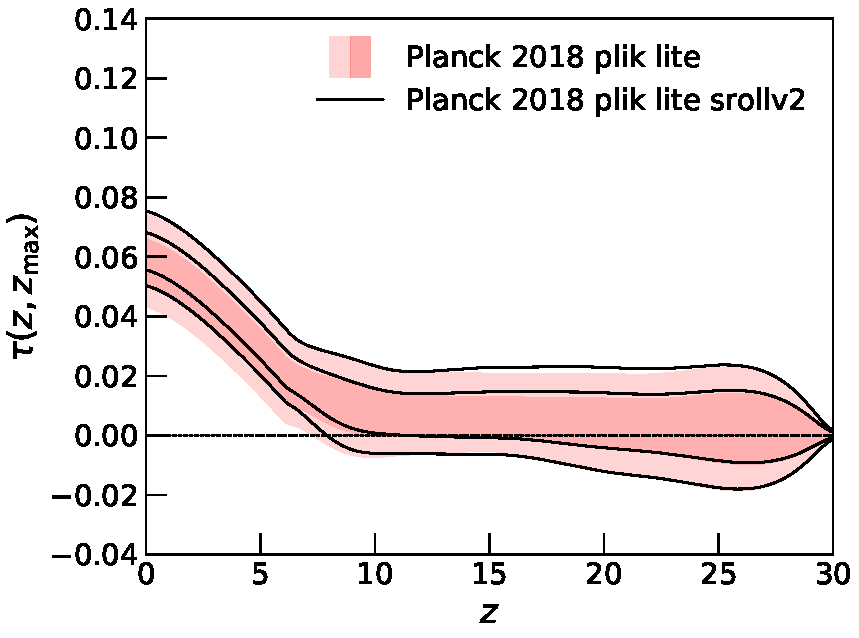
\includegraphics[width=0.45\textwidth]{results/direct_mcmc/pl18_plots_zmax30/plot_pub_tau_gtz_dz_0p1_pl18_pc_zmax30_pliklite_post_0930_and_pl18_pc_zmax30_pliklite_srollv2_0930.pdf}
\caption{[placeholder] PC chains for zmax = 30. Planck 2018 srollv2 likelihood vs Planck 2015).
}
\label{fig:plot_taugtz_2015_vs_2018}
\end{figure}

\begin{figure}[ht]
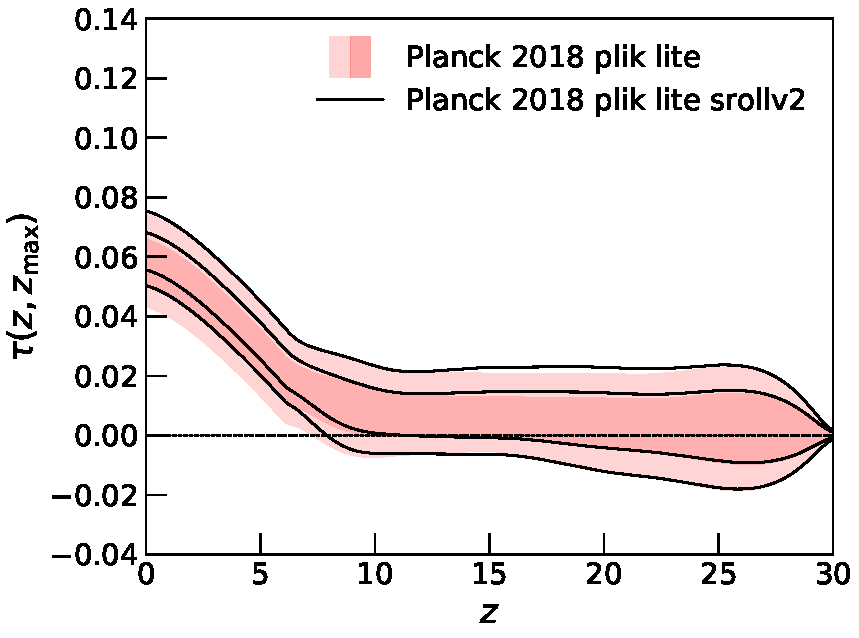
\includegraphics[width=0.45\textwidth]{results/direct_mcmc/pl18_plots_zmax30/plot_pub_tau_gtz_dz_0p1_pl18_pc_zmax30_pliklite_post_0930_and_pl18_pc_zmax30_pliklite_srollv2_0930.pdf}
\caption{PC chains for zmax = 30. Planck 2018 original lowE vs srollv2 likelihood (plik\_lite\_TTTEEE + lowl + simall\_EE vs plik\_lite\_TTTEEE + lowl + sroll2\_EE).
}
\label{fig:plot_taugtz_lowE_vs_srollv2}
\end{figure}


\begin{figure}[ht]
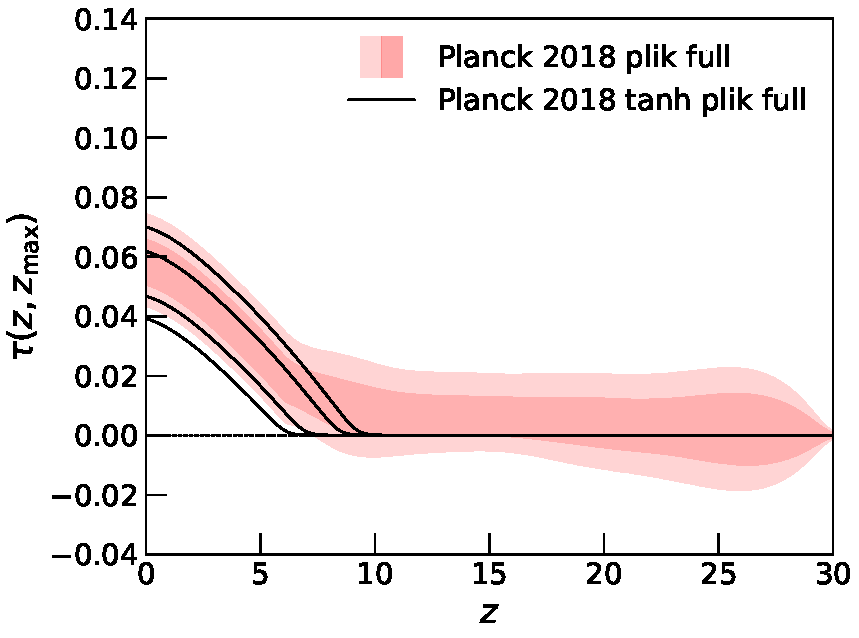
\includegraphics[width=0.5\textwidth]{results/direct_mcmc/pl18_plots_zmax30/plot_pub_tau_gtz_dz_0p1_pl18_pc_zmax30_plikfull_and_pl18_tanh_post_plikfull.pdf}
\caption{PC zmax = 30 vs tanh chains with plik\_full\_TTTEEE for the high-l likelihood.
}
\label{fig:plot_taugtz_PC_vs_tanh}
\end{figure}

\begin{figure}[ht]
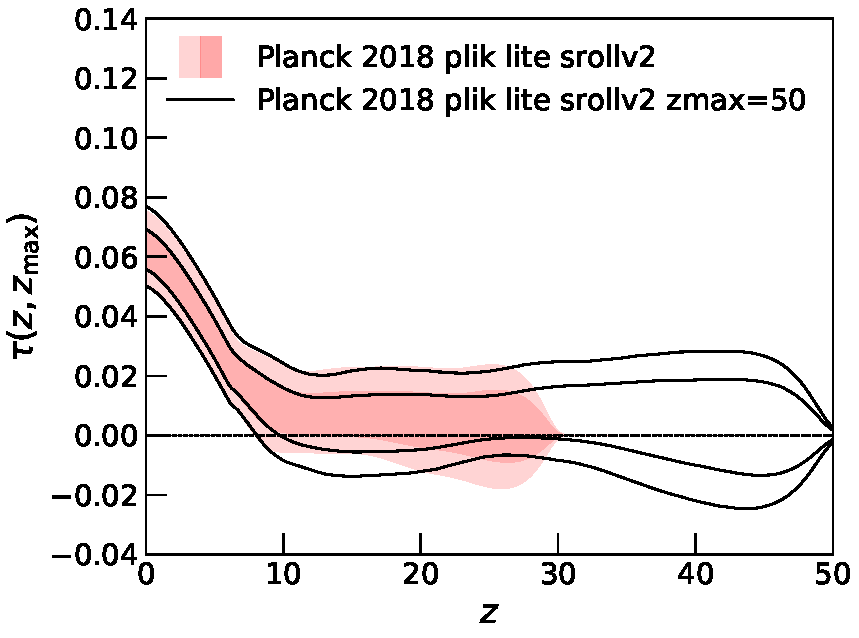
\includegraphics[width=0.45\textwidth]{results/direct_mcmc/pl18_plots_zmax30/plot_pub_tau_gtz_dz_0p1_pl18_pc_zmax30_pliklite_srollv2_0930_and_pl18_pc_zmax50_pliklite_srollv2.pdf}
\caption{Comparing zmax = 30 and 50 PC chains using Planck 2018 original lowE likelihood (plik\_lite\_TTTEEE + lowl + sroll2\_EE). Note that the zmax = 30 uses 5 PCs, whereas the zmax = 50 chains uses 7 PCs. .
}
\label{fig:plot_taugtz_zmax30_vs_zmax50}
\end{figure}


\subsection{Comparison with Previous Results}

Outline
\begin{itemize}
    \item compare with Planck official results
    \item comment that Planck tau(15,30) constraints are too stringent (flex knots). Compare to ours. Point out why.
    \item{ Comments on priors (see below).}
    \item (*maybe in  another section): make a point that dz = 0.5 for tanh may not be sufficient for experiments after Planck. This was for higher tau, so transition happens at higher redshift. Now tau is much lower.
\end{itemize}


Recap our appendix from Planck 2015 on the issue of prior:
\begin{itemize}
    \item {describe tau prior issue raised by MB18: claimed that prior not flat in tau so bias PC; proposed to flatten by multiplying the inverse of prior point-by-point in the PC space; claim that this flattening removes a shift between tanh and PC results. }
    \item {summarize that we pointed it out the flaw in the logic in appendix of \cite{Heinrich:2018btc}.}
    \item{reproduce a few tests here: 1) tau12 posterior (no need to show again, point to appendix); 2) show prior boxes in m1-m2 plane (done in Fig.4) - repeat the length of lines of constant tau12 within the box describe the prior distribution. Make the point that though the line rises, the Planck data is more informative than priors in m1, m2 makes no impact on the posterior. However when inverting the prior, introduces a bias in tau.}
    \item{show test of explicitly constructing a prior that's locally flat in m1-m2, show posterior almost doesn't change. (only change is low-z enhancement, due to prior cut off at $z>6$. between our two priors, things don't change as much (might want to reproduce this result for this Planck 2018 results. And marius version too?}
    \item{inversion method should not be used on future dataset, since data is more informative than prior.}
\end{itemize}



 
 \begin{figure}
          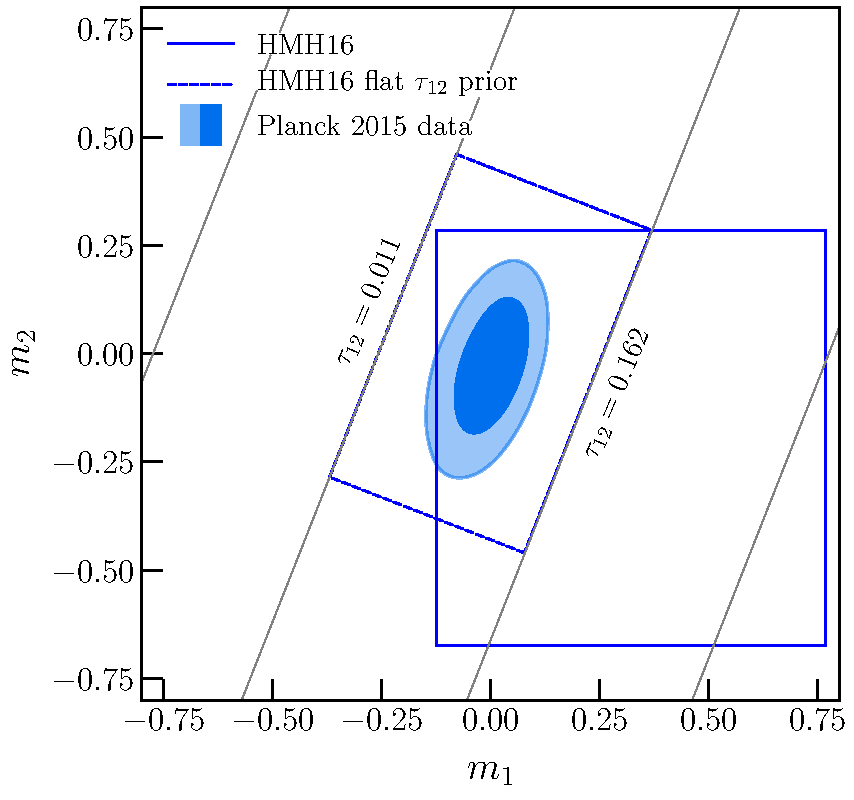
\includegraphics[width=0.9\columnwidth]{paper/plots/plot_rotated_box_flat_tau_prior_fac_0p8.pdf}
          \caption
          {[Placeholder right now (Planck 2015 plot)] Priors on the $m_1-m_2$ parameter space: the original HMH16 prior (inset square, solid lines) and a prior that is flat in
          both $\tau_{12}$ and $m_1-m_2$ (rotated rectangle, dashed lines) whose sides are aligned with lines of
          constant $\tau_{12}$ (light gray lines).   The HMH16 prior allows more parameter space at high vs low $\tau_{12}$ but this
          is not relevant since the data constraints (ellipses) exclude this region.  In the allowed region, the only difference is that the HMH16 prior clips the low $m_1$ edge of the allowed region due to physicality and the assumption that reionization occurs at
          $z\ge 6$. [add in text the comparison of priors, and how tau is not biased, and for KDE physical models determine the priors]}  \label{fig:prior_box}
\end{figure}


[Plot: add plot for tau(>z) contours for the 2 parameter model vs PC; direct integration first]

\begin{figure}
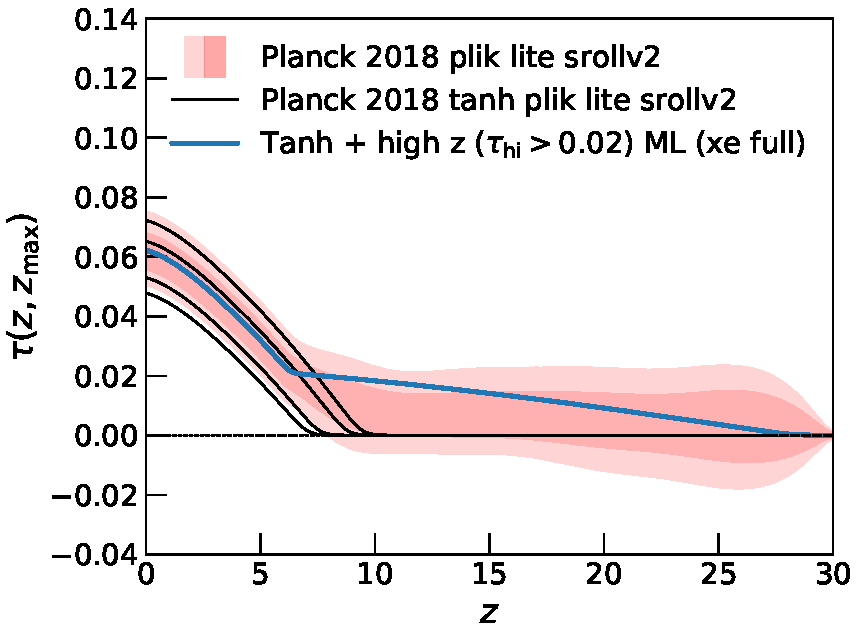
\includegraphics[width=0.40\textwidth]{plots/plot_tau_gtz.pdf}
\caption{...
}
\label{fig:}
\end{figure}


\begin{figure}
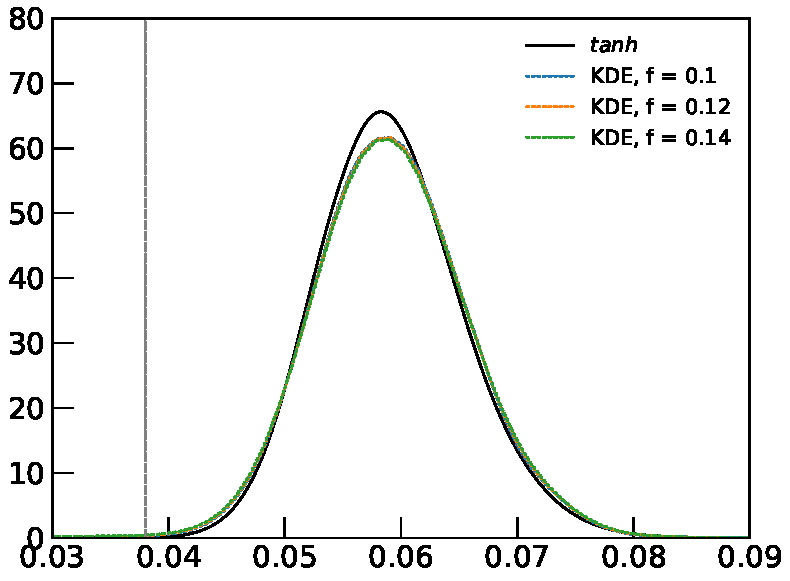
\includegraphics[width=0.40\textwidth]{plots/pl18_pc_zmax30_pliklite_srollv2_1015_tau_posterior_fraccov_1p0_burnin_10000_yes_norm_gaussian0p1_0p12_0p14.pdf}
\caption{...
}
\label{fig:}
\end{figure}



%%%%%%%%%%%%%%%%%%%%%%%%%%%%%%%%%%%%%%%%%%%%

\section{Effective Likelihood}
\label{sec:effective_likelihood}

\subsection{Code description}
\label{sec:code}

\subsection{Example 1: tanh model}
\label{sec:example1}

In Fig.~\ref{fig:reion_models}, we show the fiducial ionization history (thick blue) and contrast it with
the standard approach of CAMB (thin black) that takes hydrogen and singly ionized helium reionization to be given by
the tanh form
 \begin{equation}
x_e^{\rm true}(z) = \frac{1+f_{\rm He}}{2}\left\{  1+ \tanh\left[ \frac{y(z_*)-y(z)}{\Delta y} \right] \right\},
 \label{eqn:tanh}
 \end{equation}
 with $y(z)=(1+z)^{3/2}$, $\Delta y=(3/2)(1+z)^{1/2}\Delta z$, and $\Delta z = 0.5$.  We take here $z_*= 9.85$, corresponding the chain maximum likelihood (ML) model ($\tau = 0.0765$) from \S \ref{sec:MCMC},  for illustrative purposes.   Projected onto 5 PCs and resummed into $x_e(z)$, Eq.~(\ref{eq:mmutoxe}) yields a poor reconstruction of the ionization history itself.
 Nonetheless as we shall see in Fig.~\ref{fig:clee}, the PC decomposition provides an 
 excellent representation of the polarization power spectrum.
 

\subsection{Example 2: high-z model}
\label{sec:example2}
[rewording needed]
Our example is a two-step model 
 \bea
x_e^{\rm true}&(z)&\,= \frac{1+f_{\rm He} - \xemin}{2}\left\{  1+ \tanh\left[ \frac{y(z_{\rm re})-y(z)}{\Delta y} \right] \right\} \notag \\
&+& \frac{\xemin - x_e^{\rm rec}}{2}\left\{  1+ \tanh\left[ \frac{z_{\rm t}-z}{\Delta z_{2}} \right] \right\} + x_e^{\rm rec},
 \label{eqn:tanh_highz}
 \eea
where $y(z)=(1+z)^{3/2}$, $\Delta y=(3/2)(1+z)^{1/2}\Delta z_1$, with $\Delta z_1 = 0.25$ instead of the usual $\Delta z_1 = 0.5$,
to provide sharper distinctions between the two steps.
We choose the second step to have $z_{\rm t}=28$  and  $\Delta z_2 = 1.0$  to illustrate below
how the 5 PC analysis with $\zmax=30$ represents the same model.  Here $x_e^{\rm rec}$ is the ionization history from recombination only.
The canonical tanh model is essentially recovered in the limit $\xemin$ approaches the negligible $x_e^{\rm rec}$.  Therefore the double
step model adds a single parameter to control the high-$z$ ionization plateau for $z_{\rm re} \lesssim z \lesssim z_t$.   We show an example
of the two-step model in Fig.~\ref{fig:two_step_model}.


\begin{figure}
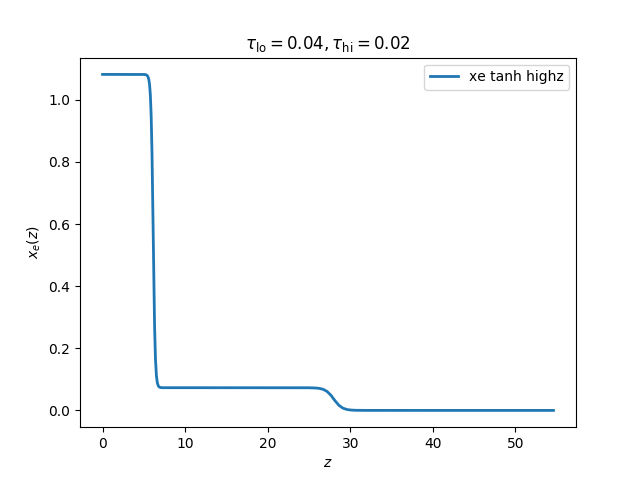
\includegraphics[width=0.5\textwidth]{results/cosmomc_kde/taulo_prior_test/plot_xez_taulo_0p04_tauhi_0p02.png}
\caption{Testing \taulo prior -- Full $x_e(z)$ of the model (\taulo, \tauhi) = (0.04, 0.02) shown in the Fig.~\ref{fig:taulo_prior_test_cl}. 
}
\label{fig:two_step_model}
\end{figure}

\begin{figure}
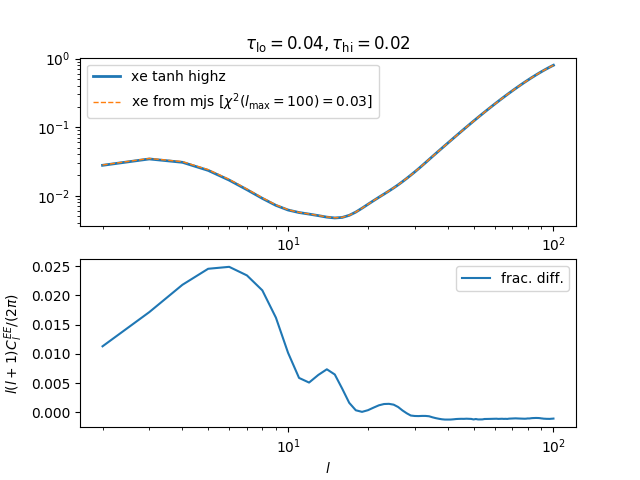
\includegraphics[width=0.5\textwidth]{results/cosmomc_kde/taulo_prior_test/plot_cls_taulo_0p04_tauhi_0p02.png}
\caption{Testing \taulo prior -- testing that \taulo $\geq$ 0.04 as \taulo prior is OK, by calculating $\chi^2$ between $C_l$ from full $x_e(z)$ vs PC decomposition of the model (\taulo, \tauhi) = (0.04, 0.02). 
The $\chi^2 = \sum_{2}^{l_{\rm max}} (\Delta C_l^{EE})^2 / \mathrm{Cov}_l = 0.03$ where $\mathrm{Cov}_l = 2 (C_l^{EE})^2/(2l+1)$. } 
\label{fig:taulo_prior_test_cl}
\end{figure}



\begin{figure}
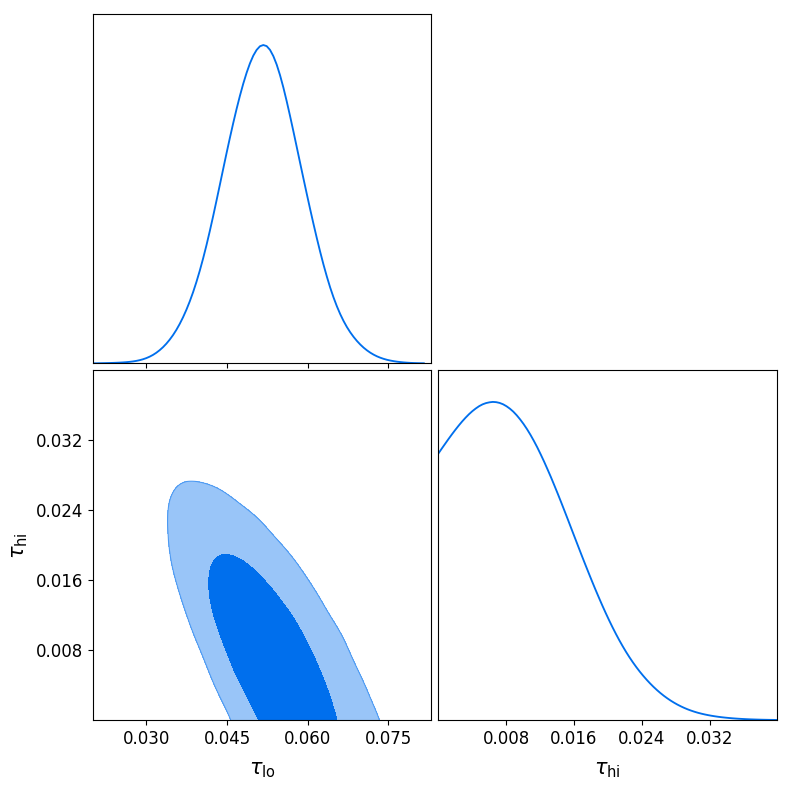
\includegraphics[width=0.5\textwidth]{results/direct_mcmc/two_parameter_model/tauhi_taulo_chains/pl18_tanh_highz_test2_run1_tri.png}
\caption{Direct MCMC chains of the two-parameter model with \tauhi and \taulo: triangle plot of \tauhi and \taulo. The marginalized 1D constraints are \taulo = $0.0516 \pm 0.0076$, \tauhi = $0.0100 \pm   0.0066$. The ML model is \taulo = 0.0543 and \tauhi = 0.0054 corresponding to $z_{\rm re} = 7.68$ and $x_{e, \mathrm{min}} = 0.021$.
}
\label{fig:two_parameter_model_2D_plot}
\end{figure}


\section{Conclusion}
\label{sec:conclusion}


\bibliography{rei.bib}

\appendix

\section{Outline (in progress)}

\begin{enumerate}
    \item{Intro}
        \begin{enumerate}
            \item 1st paragraph: CMB, reionization, why important
            \item discuss modeling of ionization history in CMB inference, tanh vs PCs (fail to capture high-z; PC captures complete parameter space), mention flex knots/other methods; cite previous PC works.
            \item give context about Planck final results; latest srollv2 likelihood, important to harness all information available, PC allows us to do that and turn into an effective likelihood.
            \item this is what we did: we obtain PC results for Planck 2018, and turn PC chains into a effective likelihood for ionization history: highlight key points like fast inference, entire model space up to zmax 30, code publicly available.
            \item we also compared to Planck official results, which is over stringent at high z, which gives additional motivations for using this likelihood; verified no hint of ionization at z>30; state any additional results.
            \item break down of sections.
        \end{enumerate}

	\item{Background}
		\begin{itemize}
			\item{Reionization Principal Components}	
			\item{Kernel Density Estimate}
		\end{itemize}
	\item{Planck 2018 PC results:\\
		- can discuss discrepancy here on high-redshift tau($>$15) constraints.\\
		- compare with our own 2015 PC results
		- zmax = 30 vs 50}
	\item{Effective Likelihood}
		\begin{itemize}
			\item{Code Description}
			\item{Examples - one and two parameter models}
		\end{itemize}
	\item{Discussion}
		
\end{enumerate}

------ \textbf{Some Numbers} ------ \\

\textbf{Planck official results 2015, 2016, 2018} \\

\begin{itemize}
    
    \item Planck 2015 results (LFI): $\tau = 0.067 \pm 0.022$ (68\%) \\

    \item Planck 2016  intermediate results (LFI): $\tau = 0.055 \pm 0.009$ (68\%) \\
    
    \item Planck 2018 results: $\tau = 0.0506 \pm 0.0086$ (68\%) \\

\end{itemize}

\textbf{Planck 2018 paper} \\

Here lowE means lowE data only, fixing all other cosmological parameters including $A_s e^{-2\tau}$\\

\begin{itemize}

\item $\tau = 0.0519+0.0030-0.0079$ (lowE; flat $\tau$ prior; TANH)(68\%); \\

\item $\tau = 0.0504+0.0050
-0.0079$ (lowE; flat $\tau$ prior; FlexKnot)(68\%); \\

\item $\tau = 0.0487+0.0038
−0.0081$ (lowE; flat $\tau$ prior; PCA)(68\%).

\end{itemize}

\textbf{Upper limit on high-redshift optical depth} (only given for the FlexKnot method):

$\tau(15, 30) < 0.006$ (lowE, flat $\tau(15, 30)$, FlexKnot); \\

$\tau(15, 30) < 0.007$ (lowE, flat knot, FlexKnot).\\

Statements to address:

\begin{enumerate}
    \item {\textbf{Statement on prior in Planck 2018}:  ``Heinrich & Hu (2018) construct a prior that is uniform on τ, but which increases the allowed unphysical parameter space and is chosen a posteriori. Here we instead use the flat prior constructed by the procedure described in Millea & Bouchet (2018) and Handley & Millea (2019), which does not admit extra unphysical models and gives the most generic prior that leaves the prior on $\tau$ uniform."}
    
    \item {Is this statement on tanh in Planck 2018 paper correct?} `` The TANH result gives slightly higher optical depth than the others, which is primarily driven by the fixed duration of reionization assumed."} \\
    
    \item{\textbf{Other comments on our PC prior giving higher optical depth}: ``The PCA result is slightly lower, and is partly affected by the imperfect physicality priors that allow unphysical negative ionization fractions." and ``Millea \& Bouchet showed that the majority of this (2$\sigma$) preference disappeared when using the lower-noise Planck HFI SimLow likelihood (intermediate results reduction of systematics), with an additional sub-dominant effect due to the choice of prior."}
    
\end{enumerate}

How likelihoods and systematics evolved over time:

\begin{enumerate}
    \item 
    \item {Planck 2018 paper attribute the 2018 upper limit on $\tau(15, 30)$ being \textbf{about 3 times more} stringent than the intermediate results by Millea \& Bouchet to the $SimLow \rightarrow SimAll$ where there was better control of systematics in HFI polarization.}
\end{enumerate}


[high redshift going away should be attributed to better control of systematics in HFI polarization data (changes in the SimAll likelihood compared to SimLow) [cite Planck 2018 results cp]]


\end{document}
